\subsection{Übertragen der Config Files mittels USB}
Um dem Programm die neuesten Konfigurationsdateien zu übergeben, steckt man beim Bootvorgang des Raspberry Pi einen Datenträger (\zB USB-Stick) an. Auf dem Datenträger muss im Root-Verzeichnis (\textasciitilde) ein Verzeichnis namens \enquote{RLT\_Config} sein. Wenn dieses Verzeichnis und alle nötigen Konfigurationsdateien (vgl. Kapitel \ref{json_config_files}) darin vorhanden sind, werden diese in das Documents Verzeichnis des Raspberry Pi kopiert. Folgendes Aktivitätsdiagramm verdeutlicht diesen Vorgang (Siehe Abb.~\ref{fig:config_ubertragen_activity}).
\begin{figure}[H]
	\centering
	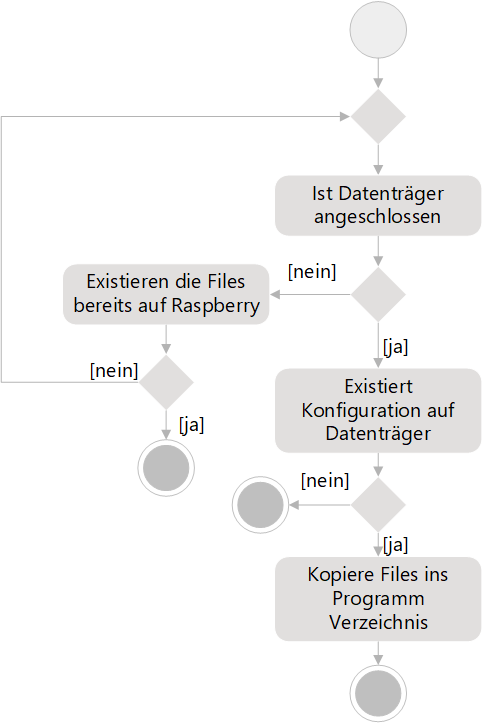
\includegraphics[width=0.4\linewidth]{Bilder/config_ubertragen_activity_diagram}
	\caption{Übertragen der Konfigurationsdateien}
	\label{fig:config_ubertragen_activity}
\end{figure}

Der Kopierablauf wird in der \enquote{usb\_routine} Funktion gestartet. Diese Funktion liefert einen Fehlercode zurück, der daraufhin in einer Verzweigung abgefragt wird. Wenn ein Fehler beim Übertragen auftritt, terminiert das Programm. Ansonsten fährt das Programm fort.
\begin{pythoncode}
if __name__ == "__main__":
	copy_error = usb_detection.usb_routine()
	if copy_error:
		exit
	all_pages = modbus.load_config()
	global app
	app = App(all_pages)
	setup_buttons()
	modbus.data_threading(app)
	app.mainloop()	
\end{pythoncode}

In der \enquote{usb\_routine} Funktion wird die \enquote{copy\_from\_usb} Funktion aufgerufen. Diese gibt einen Statuscode zurück. Die \enquote{start\_window} Funktion erstellt ein neues customtkinter Fenster, in dem dann die als Parameter angegebene Zeichenkette angezeigt wird. Das Fenster bleibt für sieben Sekunden offen, bevor es wieder geschlossen wird und die Ausführung fortfährt. Die \enquote{usb\_routine} Funktion dient als Zwischenschritt, damit der Benutzer eine Rückmeldung bekommt, ob die Konfigurationsdateien erfolgreich kopiert wurden oder keine Änderung vorgenommen wird.

\begin{pythoncode}
def usb_routine():
	copy_status = copy_from_usb()
	if copy_status == -1:
		return True # Kein Fehler
	elif copy_status == 0:
		start_window("Config Dateien wurden kopiert. Entferne nun den USB")   
	elif copy_status == 1: 
		start_window("Kein USB-Stick gefunden und Config bereits vorhanden")  
	return False # Fehler
\end{pythoncode}

Es gibt eine Hilfsfunktion namens \enquote{start\_window}, mit der Meldungen in einem Pop-Up Fenster angezeigt werden können. Dabei wird eine \enquote{Tk} Instanz erstellt, welches ein customtkinter Fenster darstellt. Zuerst wird die Überschrift, der Vollbildmodus und die Hintergrundfarbe des Fensters konfiguriert. Danach wird ein neues Label erstellt. Als Textinhalt wird der Parameter message zugewiesen. Das Fenster schließt sich nach 7 Sekunden wieder, denn customtkinter bietet die Möglichkeit eine Funktion nach Ablauf einer eingestellten Zeit auszuführen. Hier wird eine Lambda Funktion übergeben, die die \enquote{Tk} Instanz namens \enquote{msg\_window} zerstört.
\begin{pythoncode}
def start_window(message):
	msg_window = tk.Tk()
	msg_window.title("Meldung")
	msg_window.attributes('-fullscreen', True)	
	ctk.set_appearance_mode("Light")
	msg_window.configure(background="white")
	
	label = ctk.CTkLabel(master=msg_window, text_color="red", font = ('Roboto', 26), text=message, wraplength=450)
	label.place(relx=0.5, rely=0.5, anchor=tk.CENTER)
	msg_window.after(7000, lambda: msg_window.destroy())
	msg_window.mainloop()
\end{pythoncode}

Es folgt die Beschreibung der \enquote{copy\_from\_usb} Funktion. Darin wird überprüft, ob auf einem der \enquote{sd...} Ports (USB-Ports in Linux) ein Datenträger angeschlossen ist. Wenn ja, wird der entsprechende Port gespeichert und die Abfrage beendet. Die auszuführenden CLI Befehle wurden von folgender Quelle bezogen \cite{Rendek:2023}. Wenn kein Datenträger gefunden wird, kann man davon ausgehen, dass keine Änderung an der Konfiguration vorgenommen werden soll. Es wird in diesem Fall überprüft, ob im Programmverzeichnis alle benötigten Konfigurationsdateien vorhanden sind. Das passiert in der \enquote{check\_if\_files\_exists} Funktion. Wenn die Dateien bereits vorhanden sind, wird 1 zurückgegeben. Wenn die Dateien nicht vorhanden sind, wird der Vorgang wiederholt, bis ein Datenträger gefunden wird. Die Ausführung wird nach jeder Iteration für sieben Sekunden gestoppt, da die \enquote{check\_if\_files\_exists} Funktion ein Meldungsfenster öffnet und dieses sieben Sekunden lang die weitere Ausführung verhindert. Dadurch hat der Benutzer oder die Benutzerin genügend Zeit um einen Datenträger einzufügen.

\begin{pythoncode}
	port = ""
	while True:
		if (os.system("mount | grep sda1") != 256):
			port = "sda1"
			break
		elif (os.system("mount | grep sdb1") != 256):
			port = "sdb1"
			break
		elif (os.system("mount | grep sdc1") != 256):
			port = "sdc1"
			break
		elif (os.system("mount | grep sdd1") != 256):
			port = "sdd1"
			break
		
		if (check_if_files_exists(config_path, device_config_path, False)):
			return 1
\end{pythoncode}

Wenn ein Datenträger gefunden wurde, wird der vorher gespeicherte Port gemountet. Nun wird überprüft, ob die notwendigen Konfigurationsdateien auf dem Datenträger existieren. Wenn nicht, wird der Datenträger ausgeworfen und ein Fehlercode zurückgegeben. Ansonsten werden die Dateien vom USB-Stick ins Programmverzeichnis kopiert und der Datenträger entmountet. 
\begin{pythoncode}
	os.system("sudo umount /dev/" + port)
	os.system("sudo mount /dev/" + port + " /home/pi/Documents/Config")
	
	error_free = check_if_files_exists(usb_config_path, usb_device_config_path, True)
	if error_free:
		os.system("cp -r ~/Documents/Config/RLT_Config ~/Documents/")
	else:
		os.system("sudo umount /dev/" + port)
		return -1
		
	os.system("sudo umount /dev/" + port)
	return 0
\end{pythoncode}

Nachdem der \enquote{umount} Befehl ausgeführt und der Datenträger physisch entfernt wird, erscheint auf dem Display eine Warnung, dass der Datenträger entfernt wurde, ohne ausgeworfen worden zu sein. Ausprobiert wurde auch der folgende Befehle, allerdings erschien immer noch die selbe Warnung \cite{Totor:2022}.
\begin{pythoncode}
	os.system("sudo eject /dev/" + port)
\end{pythoncode}
Die Erkenntnis ist, dass hier das unmounten ausreichend ist und die Warnung ignoriert werden kann, da diese in diversen Testversuchen keine unerwünschten Nebenwirkungen verursachte. Außerdem stört sie auch nicht die Benutzerfreundlichkeit, da die \acs{gui} im Vollbild ausgeführt wird und somit die Warnung verdeckt.

Zweimal muss an unterschiedlichen Stellen überprüft werden, dass die Konfigurationsdateien existieren. Dafür gibt es die Funktion \enquote{check\_if\_files\_exists}. Diese erhält als Parameter zuerst eine Zeichenkette, die den Pfad zum Speicherort der Konfigurationsdateien auf dem externen Datenträger angibt. Außerdem eine Zeichenkette, die den Pfad zum Speicherort des devices Unterordner angibt. Es wird nun also überprüft, ob an dem angegebenen Pfad tatsächlich das Verzeichnis \enquote{RLT\_Config} existiert. Danach wird überprüft, ob die Hauptkonfigurationsdatei darin existiert. Danach wird überprüft, ob ein Unterordner namens \enquote{devices} existiert. Schließlich wird noch überprüft, ob die Sensors Konfigurationsdatei im devices Ordner existiert. Die Existenz bestimmter Gerätekonfigurationsdateien kann nicht geprüft werden, da die Dateinamen variabel und abhängig vom Gerätetyp sind (z.B. QBM97XX, EBM). Nach jeder fehlgeschlagenen Überprüfung wird ein Fenster geöffnet, auf dem eine genauere Fehlerherkunft beschrieben steht, damit der Administrator bzw. die Administratorin den Fehler einfacher beheben kann.
\begin{pythoncode}
def check_if_files_exists(config_path, device_config_path):
	if not os.path.exists(config_path):
		start_window("RLT_Config Ordner existiert nicht")
		return False
	if not os.path.isfile(config_path + "main_config_file.json"):
		start_window("main_config_file.json existiert nicht")
		return False
	if not os.path.exists(device_config_path):
		start_window("devices Ordner existiert nicht")
		return False
	if not os.path.exists(device_config_path + "sensors.json"):
		start_window("devices/sensors.json existiert nicht")
		return False
	return True
\end{pythoncode}